\documentclass[11pt]{beamer}
\usetheme{Warsaw}
\usepackage[utf8]{inputenc}
\usepackage[english]{babel}
\usepackage{enumitem}
\usepackage{enumerate}
\usepackage{mathtools}
\usepackage{amsmath}
\usepackage{amsfonts}
\usepackage{amssymb}
\usepackage{graphicx}
\usepackage{hyperref}
\hypersetup{
    colorlinks=true,
    linkcolor=blue,
    filecolor=magenta,      
    urlcolor=blue,
}
\graphicspath{ {./images/} }
\usepackage{array}
\author{Aravind and Jeel}
\title{IDP - EE3025}
\setbeamercovered{transparent}
\setbeamertemplate{navigation symbols}{}
%\logo{} 
\institute{IIT Hyderabad} 
\date{8th March, 2019}
%\subject{} 

\begin{document}

\begin{frame}
\titlepage
\end{frame}

\begin{frame}{Project Idea: \\ Edge Detection on Images}

	Sobel Filter is used to detect two kinds of edges in an image \\
	\begin{itemize}
	\item[•] Vertical Direction
	\item[•] Horizontal Direction
	\end{itemize}
	
	% write about sobel filter
	% math equations
\end{frame}

\begin{frame}{Edge Detection on Images}
	
	\textbf{Vertical Mask}
	\begin{center}
	
	\begin{tabular}{|m{1cm}|m{1cm}|m{1cm}|}
	\hline
	-1 & 0 & 1 \\
	\hline
	-2 & 0 & 2 \\
	\hline
	-1 & 0 & 1 \\
	\hline
	
	\end{tabular}
	\end{center}
	\pause
	\textbf{Horizontal Mask}
	\begin{center}
	
	\begin{tabular}{|m{1cm}|m{1cm}|m{1cm}|}
	\hline
	-1 & -2 & -1 \\
	\hline
	0 & 0 & 0 \\
	\hline
	1 & 2 & 1 \\
	\hline
	
	\end{tabular}
	\end{center}
	
	% write about sobel filter
	% math equations
\end{frame}

\begin{frame}
\textbf{Sample image}
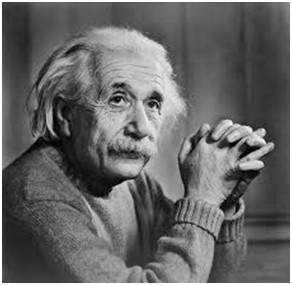
\includegraphics{sobel1}
\end{frame}

\begin{frame}
\textbf{After applying vertical mask}
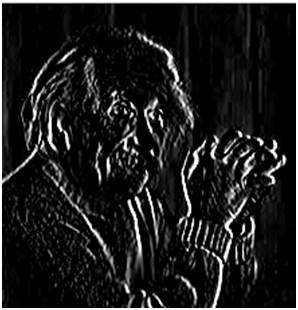
\includegraphics{sobel2}
\end{frame}

\begin{frame}
\textbf{After applying horizontal mask}
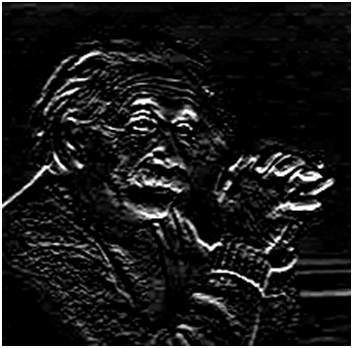
\includegraphics{sobel3}
\end{frame}

\begin{frame}{Implementation Plan}
	\begin{itemize}
		\item[•] {Load image into FPGA
			\begin{itemize}
				\item[\rightarrow] Convert image to hex file using \textit{ffmpeg}
				\item[\rightarrow] Stream these pixel values as bytes from Raspberry Pi to FPGA RAM using \textit{ffmpeg}
				\item[\rightarrow] Write a coordinate decoder module on sequence of pixels (bytes). For this we need to specify the image size. We plan to use pilot bytes to detect row endings in later stages of the project. 
			\end{itemize}
		}
		\pause
		\item[•] { To Implement an efficient Sobel Filter on FPGA
			\begin{itemize}
				\item[\rightarrow] Efficient Convolution algorithm of an image of known shape with a known constant filter 
			\end{itemize}
		}
	\end{itemize}

\end{frame}

\begin{frame}{References}
\begin{itemize}
\item \href{https://github.com/jhol/otl-icoboard-pmodoledrgb-demo}{https://github.com/jhol/otl-icoboard-pmodoledrgb-demo}
\item \href{https://en.wikipedia.org/wiki/Sobel_operator}{\text{https://en.wikipedia.org/wiki/Sobel\_operator}}
\end{itemize}

\end{frame}

\end{document}
